\section{Package Entities}

\begin{figure}[H] 
    \centering 
    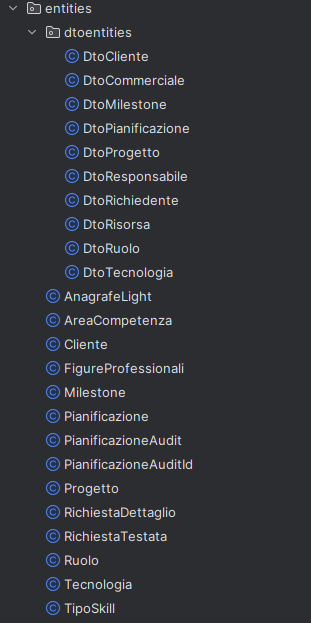
\includegraphics[width=0.4\columnwidth]{entities-package2} 
    \caption{Package entità}
\end{figure}

\noindent All'interno del package Entities troviamo le entità. Per entità si intendono tutte quelle classi Java che definiscono i modelli di dati dell'applicazione.\\
Queste classi vengono annotate con annotazioni JPA utili a stabilire come la classe venga associata a una tabella presente nel database relazionale. Ogni istanza di un'entità rappresenta una riga nella tabella relativa.\\
Di tutte le tabelle da me create è stata mappata ogni relazione tra tabelle e campo, mentre per ogni tabella del database aziendale sono stati mappati tutti i campi e le relazioni ad altre tabelle che potevano tornarmi utili.\\
In ogni entità troviamo setters e getters, costruttori con e senza argomenti.\\

\subsection{Esempio di un'entità}
\begin{figure}[H] 
    \centering 
    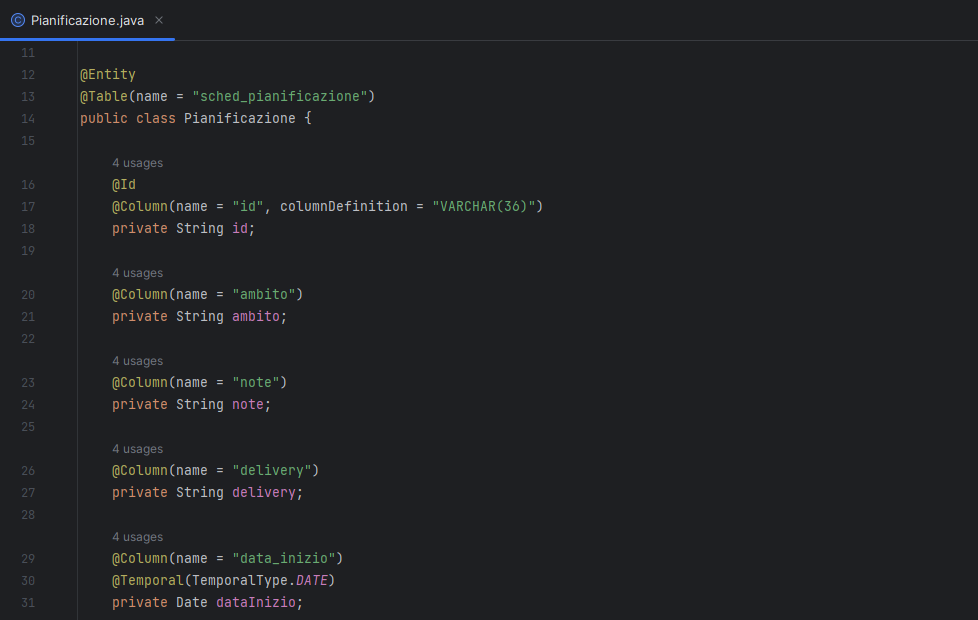
\includegraphics[width=0.9\columnwidth]{esempio-entita} 
    \caption{Esempio di mappatura di un'entità}
\end{figure}

\noindent Nell'immagine qui sopra possiamo notare uno snippet dell'entità Pianificazione in cui sono state utilizzate le seguenti annotazioni:
\begin{itemize}
\item \textit{@Entity}, per mappare le classi Java che rappresentano una tabella in un database, si inserisce questa notazione specificandola a class level\textsubscript{g}.
\item \textit{@Table}, nella maggior parte dei casi il nome di una tabella nel database e il nome dell'entità non sono gli stessi. Per questo motivo è stata utilizzata la seguente annotazione per specificare il nome della tabella;
\item \textit{@Column}, utilizzata per mappare una campo di una classe a una colonna di una tabella nel database. Questa annotazione ha dei parametri, come ad esempio "name", che serve a specificare il nome della colonna a cui è associato il campo;
\item \textit{@Id}, per identificare un campo all'interno di una classe che mappa la chiave primaria di una tabella del database viene utilizzata questa annotazione;
\item \textit{@Temporal}, utilizzata per specificare se un campo di tipo Date dovrebbe essere mappato come \textit{TemporalType.DATE}, per una data senza orario, \textit{TemporalType.TIME} per un orario senza data e infine \textit{TemporalType.TIMESTAMP}, utilizzato nella tabella di log di Pianificazione per mappare un campo con data e orario.
\end{itemize}
\subsection{Mappatura delle relazioni}
\begin{figure}[H] 
    \centering 
    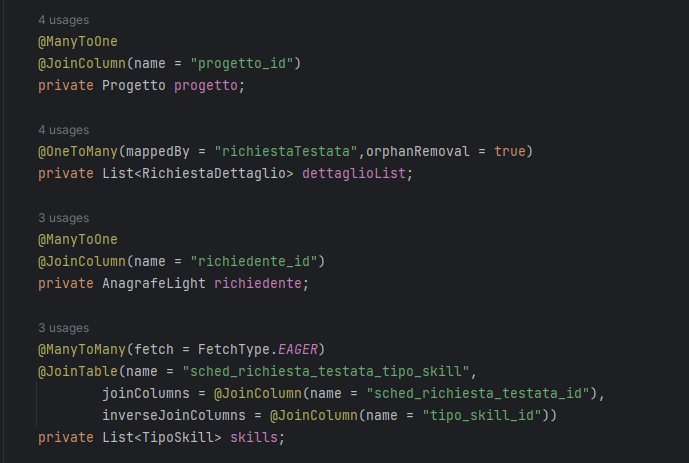
\includegraphics[width=0.9\columnwidth]{esempio-relazioni} 
    \caption{Esempio di mappatura delle relazioni della tabella RichiestaTestata}
\end{figure}
\noindent Per mantenere le relazioni tra le tabelle sono state utilizzate annotazioni che si possono osservare nel code snippet qui sopra raffigurante una porzione della classe Java che mappa la tabella RichiestaTestata.\\
Nel caso in cui sia necessario che entrambi i lati di una relazione debbano accedere all'informazione, viene dichiarata una relazione bidirezionale. In questo contesto, è fondamentale gestire correttamente la sincronizzazione tra le due entità.
\begin{itemize}
\item \textbf{uno-a-molti}, relazione in cui il campo associato sarà una lista di oggetti della classe opposta (in relazione all'esempio, una RichiestaTestata è associata a più RichiesteDettaglio), mentre nella relazione molti-a-uno sarà un oggetto singolo della classe opposta annotato con \textit{@JoinColumn} con "name" uguale a quello del campo nella tabella del database (in relazione all'esempio, una RichiestaTestata ha un solo Richiedente).\\
Nell'esempio è stato utilizzato il parametro \texttt{mappedBy} per mappare la relazione opposta e \texttt{orphanRemoval} per poter implementare la cancellazione di una RichiestaTestata garantendo l'eliminazione di tutte le RichiesteDettaglio associate al momento della rimozione.
\item \textbf{uno-a-uno}, relazione in cui un record della tabella è associato ad un solo record dell'altra tabella. Anche in questo caso se si vuole mappare da entrambi le parti la relazione bisogna utilizzare lo stesso principio dichiarato nella relazione precedente, solo che entrambe le parti avranno come campo un oggetto della classe opposta.\\
Non sono state identificate relazioni uno-a-uno nel database.
\item \textbf{molti-a-molti}, relazione in cui viene mappata la tabella di join presente nel database tra le due tabelle, utilizzando il codice che si vede in esempio.
Per gestire operazioni di rimozione tra le due tabelle è stato utilizzato un metodo annotato con \textit{@PreRemove} nella classe \texttt{TipoSkill}, che entra in azione quando una RichiestaTestata viene eliminata, assicurando che la disconnessione avvenga in modo appropriato.
%\item \textbf{relazione bidirezionale}, relazione in cui è importante gestire correttamente la sincronizzazione tra le due direzioni della relazione, dato che quando si aggiorna una parte dell'entità bisogna aggiornare anche l'altra. Per mappare una relazione non è necessario mappare entrambi i lati della relazione, ma ritorna utile solo in base quello che si va ad implementare.
\end{itemize}
\subsection{Subpackage dtoentities}
All'interno del package "dtoentities" troviamo tutte quelle classi DTO delle entità di cui servivano soltanto determinate informazioni da restituire all'utente, evitando così ridondanza o informazioni superflue. Queste classi non contengono annotazioni, ma sono semplicemente degli oggetti contenenti i campi semplificati delle entità. A loro volta possono contenere altri DTO di altre entità in base alle relazioni che hanno.
\begin{figure}[H] 
    \centering 
    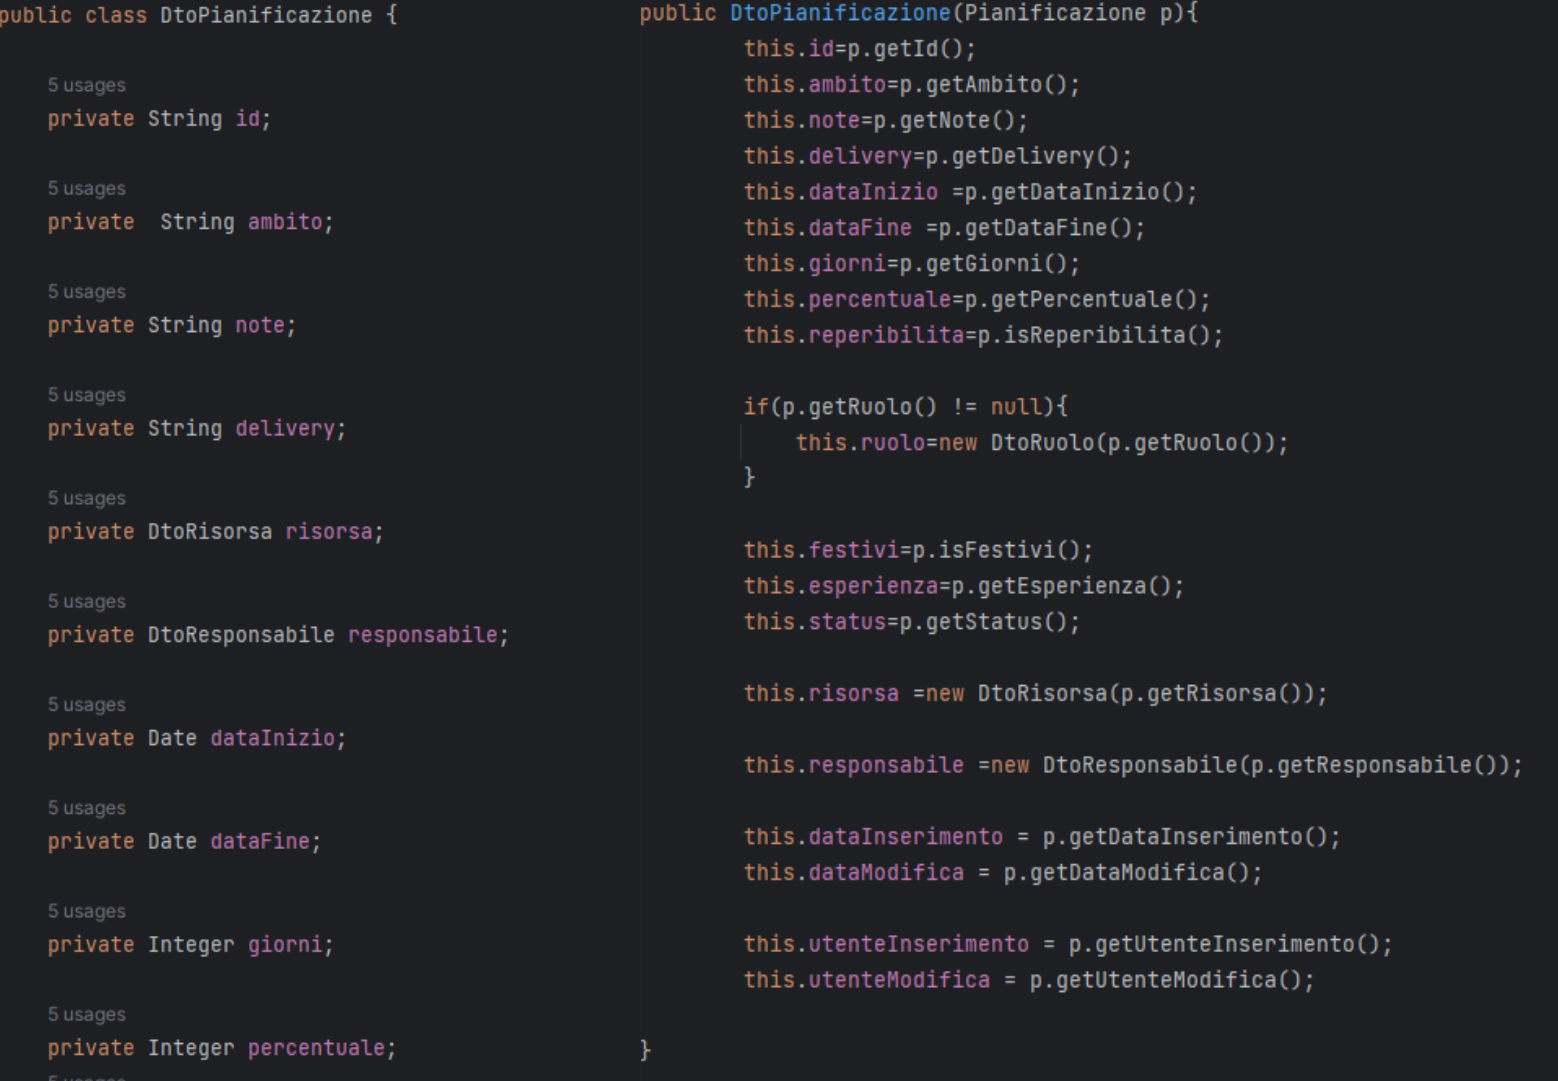
\includegraphics[width=0.9\columnwidth]{merge-dtopianificazione} 
    \caption{Esempio di classe DTO di Pianificazione}
\end{figure}
\noindent Ogni entità DTO possiede tre costruttori: costruttore senza argomenti e con argomenti e infine un costruttore che velocizzava la conversione da entità ad entità DTO (come mostrato nell'immagine qui sopra).